\chapter{Band Theory of Metals}
In Chapter \ref{ch:solids}, we showed how all the contributions of all the valence ions/electrons/..., kinetic energies and interactions between the particles could be written as a one electron Schrödinger equation. Some approximations made to achieve this are: Born-Oppenheimer apporximation, Hartree approximation and the static approximation.
The one electron Schrödinger equation states:
\begin{equation}
	\left[-\frac{\hbar^2}{2m}\nabla^2 + V(\vec{r})\right]\psi(\vec{r}) = E\psi(\vec{r}) \label{eqn:schrodinger_tbu}
\end{equation}
As we know, this potential is called the crystal potential energy fucntion. It has periodic properties. Now, we can deduce properties, originating from the periodicity of $V(\vec{r})$, af this Schrödinger equation.

\section{Property 1: Influence of translation operator on the Schrödinger equation} \label{sec:property1}
\dfn{Translation operator}{What is a translation operator: \begin{equation} \hat{T}_{\vec{R}}f(\vec{r}) = f(\vec{r} + \vec{R}) \end{equation}}
\nt{We put a hat ( $\hat{}$ ) on the letter to show that it is a operator.}
Applying this on the Schrödinger equation result in:
\begin{align}
	\hat{T}_{\vec{R}}H\psi(\vec{r}) &= \hat{T}_{\vec{R}}(H(\vec{r})\psi(\vec{r}))\\
	&= H(\vec{r} + \vec{R})\psi(\vec{r} + \vec{R})\\
	&= H(\vec{r})\psi(\vec{r} + \vec{R})\\
	&= H(\vec{r})\hat{T}_{\vec{R}}\psi(\vec{r})
\end{align}
Thus we can conclude that:
\begin{align}
	\hat{T}_{\vec{R}}H\psi &= H\hat{T}_{\vec{R}}\psi \\
	\hat{T}_{\vec{R}}H &= H\hat{T}_{\vec{R}} \\
	\left[\hat{T}_{\vec{R}}, H\right] &= 0 \label{eqn:commutation}
\end{align}
\clm{Product of translation operators}{}{The product of two translation operators can be defined as: \begin{equation} \hat{T}_{\vec{R}}\hat{T}_{\vec{R}'} = \hat{T}_{\vec{R} + \vec{R}'}  \label{prop:translation} \end{equation}}
\begin{myproof}
	We can show this by simply working out the operations on a function:
	\begin{align}
		\hat{T}_{\vec{R}}\hat{T}_{\vec{R}'}\psi(\vec{r}) &= \hat{T}_{\vec{R}}\psi(\vec{r} + \vec{R}') \\
		&= \psi(\vec{r} + \vec{R} + \vec{R}') \\
		&= \hat{T}_{\vec{R} + \vec{R}'}\psi(\vec{r})
	\end{align}
\end{myproof}
What is now so interesting about this commutation relation (equation \ref{eqn:commutation})? Well, it is linked to a fundamental property of Quantum mechanics.
\thm{Property of commutators in QM}{If $\left[\hat{T}_{\vec{R}}, H\right] = 0$ then all eigenstates of $H$ can be chosen to have the same eigenstates as $\hat{T}_{\vec{R}}$. In other words, if $H$ and $\hat{T}_{\vec{R}}$ commute, than they have a commen set of eigenstates. We will derive them here.\par
Because the translational operator has the same set of eigenstates the following set of equations are equivalent.
\begin{align}
	\left\{
	\begin{array}{lr}
		H\psi = E\psi \\
		\hat{T}_{\vec{R}}\psi = \lambda(\vec{R})\psi
	\end{array}
	\right
\end{align}
We still do not know what these $\lambda(\vec{R})$ eigenvalues belong to it, the energy states are the same.\par
Following from the property form equation \ref{prop:translation}, we can deduce some properties for $\lambda(\vec{R})$:
\begin{align}
	& \lambda(\vec{R})\lambda(\vec{R}') = \lambda(\vec{R} + \vec{R}') \\
	& \lambda^n(\vec{R}) = \lambda(n\vec{R})
\end{align}
A value that satisfies, these two conditions is:
\begin{equation}
	\lambda(\vec{R}) = e^{i\vec{k}\cdot\vec{R}} \qquad \text{with $\vec{k}$ some complex vector.}
\end{equation}
Normalisation requires that:
\begin{align}
	\int_{V}^{}\abs{\psi}^2d\vec{r} &= 1 \label{eqn:norm} \\
	\Rightarrow \int_{V}^{}\abs{\hat{T}_{\vec{R}}\psi(\vec{r})}^2d\vec{r} &= \int_{V}^{}\abs{\psi(\vec{r} + \vec{R})}^2d\vec{r} \label{eqn:norm_2} \\
	&= \int_{V}^{}\abs{\lambda(\vec{R})\psi(\vec{r})}^2d\vec{r} \nonumber \\
	&= \int_{V}^{}\abs{\lambda(\vec{R})}^2\abs{\psi(\vec{r})}^2d\vec{r} \nonumber\\
	&= \abs{\lambda(\vec{R})}^2\int_{V}^{}\abs{\psi(\vec{r})}^2d\vec{r} \nonumber \\
	&= \abs{\lambda(\vec{R})}^2 \label{eqn:simplification_integral}  \\
	&= 1 \label{eqn:lambda_simplification}
\end{align}
Step \ref{eqn:simplification_integral} is possible due to \ref{eqn:norm}. The last step (equation \ref{eqn:lambda_simplification}) follows from that is $\psi$ is normalized (equation \ref{eqn:norm}), the translation of $\psi$ is still normalized.\par
Now because of the fact that we have the normalisation (equation \ref{eqn:norm_2}), we can say that $\vec{k}$ can be written as a real vector $k_x\vec{e}_x + k_y\vec{e}_y + k_z\vec{e}_z$ with $k \in \bbR$.\par
Now because we have a periodic crystal potential, we can write the following:
\begin{equation}
	\hat{T}_{\vec{R}}\psi(\vec{r}) = e^{i\vec{k}\cdot\vec{R}}\psi(\vec{r}) \label{eqn:eigenstates_transoperator}
\end{equation}}

\section{Bloch's theorem} \label{sec:bloch}
\dfn{Block's theorem}{The Bloch's theorem states:
\begin{equation}
	\psi(\vec{r}) = u(\vec{r})e^{i\vec{k}\cdot\vec{r}} \qquad \text{where } u(\vec{r}) \text{ is periodic}
\end{equation}
$e^{i\vec{k}\cdot\vec{r}}$ is a plain wave function.}
\ex{How Bloch's theorem works}{
	\begin{align}
		\hat{T}_{\vec{R}}\psi(\vec{r}) &= \hat{T}_{\vec{R}}\left(u(\vec{r})e^{i\vec{k}\cdot\vec{r}}\right) \\
		&= u(\vec{r} + \vec{R})e^{i\vec{k}\cdot(\vec{r} + \vec{R})} \\
		\text{(if }u(\vec{r})\text{ is periodic)}\qquad &= e^{i\vec{k}\cdot(\vec{r} + \vec{R})}u(\vec{r}) \\
		\text{(using Bloch)}\qquad &= e^{i\vec{k}\cdot\vec{R}}\psi(\vec{r}) \\
		&= \lambda(\vec{R})\psi(\vec{r}) \\
		&= \hat{T}_{\vec{R}}\psi(\vec{r})
	\end{align}
}

Furthermore, you can the eigenstates of the translation operator (equation \ref{eqn:eigenstates_transoperator}), too:
\begin{equation}
	\hat{T}_{\vec{R}}\psi(\vec{r}) = \psi(\vec{r} + \vec{R}) = u(\vec{r} + \vec{R})e^{i\vec{k}\cdot(\vec{r} + \vec{R})} = u(\vec{r})e^{i\vec{k}\cdot\vec{r}}e^{i\vec{k}\cdot\vec{R}} = e^{i\vec{k}\cdot\vec{R}}\psi(\vec{r})
\end{equation}

\subsection{Closer look at the Schrödinger equation}
To identify each wavevector, we will use a $\vec{k}$ subscript referring to the plain wave in Bloch's theorem (section \ref{sec:bloch}). As it turns out the function $u(\vec{r})$ will also depend on $\vec{k}$ ($u_{\vec{k}}(\vec{r})$). We now get the following by using Bloch:
\begin{align}
	H\psi &= E\psi \\
	H\psi_{\vec{k}}(\vec{r}) &= E(\vec{k})\psi_{\vec{k}}(\vec{k})\\
	\left\{\frac{\hbar^2}{2m}\left(-i\vec{\nabla}+ \vec{k}\right)^2 + V(\vec{r})\right\}u_{\vec{k}}(\vec{r}) &= E(\vec{k})u_{\vec{k}}(\vec{r}) \label{eqn:eigvalprob}
\end{align}
We get a Schrödinger equation for the periodic function $u$. Equation \ref{eqn:eigvalprob} is an eigenvalue problem that is confined in a finite volume (the cyrstal) where $u$ has to obey to it's periodic boundary conditions $u_{\vec{k}}(\vec{r}) = u_{\vec{k}}(\vec{r} + \vec{R})$. What are the eigenvalues?\par
From differential equation analysis and eigenvalue problems we know we get a discrete set of eigenvalues: $E_n(\vec{k})$. This existence of this discrete set is because we impose boundary conditions on the problem. We can now 'update' the Schrödinger equation (\ref{eqn:eigvalprob}):
\begin{equation}
	\left\{\frac{\hbar^2}{2m}\left(-i\vec{\nabla}+ \vec{k}\right)^2 + V(\vec{r})\right\}u_{n, \vec{k}}(\vec{r}) &= E(n, \vec{k})u_{n, \vec{k}}(\vec{r}) \label{eqn:schrodinger_complete}
\end{equation}

\section{Properties of the energy eigenvalues of $u_{n, \vec{k}}$}
\clm{}{}{Both wave function and energy eigenvalues satisfy (for $\vec{G}$ a reciprocal lattice vector):
\begin{equation}
	\left\{
	\begin{array}{lr}
		E_n(\vec{k} + \vec{G}) = E_n(\vec{k}) \\
		\psi_{n, \vec{k} + \vec{G}}(\vec{r}) = \psi_{n, \vec{k}}(\vec{r})
	\end{array}
	\right
\end{equation}}
\begin{myproof}
	If we substitude the following equation into equation \ref{eqn:schrodinger_tbu}, we get \ref{eqn:updatedschrod}.
	\begin{equation}
		\psi_{n, \vec{k} + \vec{G}}(\vec{r}) = u_{n, \vec{k} + \vec{G}}(\vec{r})e^{i(\vec{k} + \vec{G})\cdot\vec{r}}
	\end{equation}
	\begin{equation}
		\left\{\frac{\hbar^2}{2m}\left(-i\vec{\nabla} + \vec{k}\right)^2 + V(\vec{r})\right\}u_{n, \vec{k} + \vec{G}}(\vec{r})e^{i\vec{G}\cdot\vec{r}} = E_n(\vec{k} + \vec{G})u_{n, \vec{k} + \vec{G}}(\vec{r})e^{i\vec{G}\cdot\vec{r}} \label{eqn:updatedschrod}
	\end{equation}
	What we see now is that from \ref{eqn:schrodinger_complete} and \ref{eqn:updatedschrod} we expect:
	\begin{equation}
		u_{n, \vec{k} + \vec{G}}(\vec{r})e^{i\vec{G}\cdot\vec{r}} = u_{n, \vec{k}}(\vec{r})
	\end{equation}
	Thereby we can say that:
	\begin{equation}
		\psi_{n, \vec{k} + \vec{G}}(\vec{r}) = u_{n, \vec{k} + \vec{G}}(\vec{r})e^{i(\vec{k} + \vec{G})\cdot\vec{r}} = u_{n, \vec{k} + \vec{G}}(\vec{r})e^{i\vec{k}\cdot\vec{r}} = \psi_{n, \vec{k}}(\vec{r})
	\end{equation}
	Now we can also show that $E_n(\vec{k} + \vec{G}) = E_n(\vec{k})$.
\end{myproof}
What you might notice now is that $\vec{G}$ can be any vector, instead of being a reciprocal lattice vector. How do we enforce this requirement? Well, because equation \ref{eqn:schrodinger_complete} and equation \ref{eqn:updatedschrod} are the same, the wavefunctions must obey the same periodic boundary conditions. That is only true if $\vec{G}$ is a reciprocal lattice vector.
We can show this has to be the case by:
\begin{align}
	\hat{T}_{\vec{R}}\left(u_{n, \vec{k} + \vec{G}}(\vec{r})e^{i\vec{G}\cdot\vec{r}}\right) &= u_{n, \vec{k} + \vec{G}}(\vec{r} + \vec{R})e^{i\vec{G}\cdot(\vec{r} + \vec{R})} \\
	&= u_{n, \vec{k} + \vec{G}}(\vec{r})e^{i\vec{G}\cdot\vec{r}}e^{i\vec{G}\cdot\vec{R}} \\
	&\Rightarrow e^{i\vec{G}\cdot\vec{R}} = 1
\end{align}

\section{Property 2: Inversion symmetry} \label{sec:property2}
\dfn{Inversion symmetry}{Inversion symmetry states that \begin{equation} E_n(-\vec{k}) = E_n(\vec{k}) \label{eqn:property2} \end{equation}}
This has an effect on a property of the wave equation:
\begin{align}
	\psi_{n, \vec{k}}^{*}(\vec{r} + \vec{R}) &= \left(\psi_{n, \vec{k}}(\vec{r} + \vec{R})\right)^{*} \\
	\text{(By equation \ref{eqn:eigenstates_transoperator})}\qquad &= \left(e^{i\vec{k}\cdot\vec{R}}\psi_{n, \vec{k}}(\vec{r})\right)^{*} \\
	&= e^{-i\vec{k}\cdot\vec{R}}\psi_{n, \vec{k}}^{*}(\vec{r})
\end{align}
The complex conjugate wavefunction still complies with Bloch's theorem, therefore we can say that:
\begin{equation}
	\psi_{n, \vec{k}}^{*}(\vec{r}) = \psi_{n, -\vec{k}}(\vec{r})
\end{equation}
Now, we proof the property for energy eigenvalues (equation \ref{eqn:property2}) by starting form the complex conjugate Schrödinger equation:
\begin{align}
	H^{*}\psi_{n, \vec{k}}^{*}(\vec{r}) = H\psi_{n, \vec{k}}^{*}(\vec{r}) &= \left(H\psi_{n, \vec{k}}(\vec{r})\right)^{*} \\
	&= \left(E_n(\vec{k})\psi_{n, \vec{k}}(\vec{r})\right)^{*} \\
	&= E_n\psi_{n, \vec{k}}^{*}(\vec{r}) \\
	\Rightarrow H\psi_{n, -\vec{k}}(\vec{r}) &= E_n(-\vec{k})\psi_{n, -\vec{k}}(\vec{r}) \\
	&= E_n(-\vec{k})\psi_{n, \vec{k}}^{*}(\vec{r}) \\
	\Rightarrow E_n(-\vec{k}) = E_n(\vec{k}) \nonumber
\end{align}

\section{Consequences of the properties}
As we saw for the Schrödinger equation:
\begin{align}
    &-\frac{\hbar^2}{2m}\nabla^2\psi_{n, \vec{k}}(\vec{r}) + V(\vec{r})\psi_{n, \vec{k}}(\vec{r}) = E_n(\vec{k})\psi_{n, \vec{k}}(\vec{r}) \\
    & \qquad \rightarrow V(\vec{r}) = V(\vec{r} + \vec{R})
\end{align}

This says something about the energy spectrum, in function of $\vec{k}$. As we see in figure \ref{fig:energybandiagram}, we have energy bands $E_i$, these all have all eigenvalues and between the bands we have bandgaps, there there aro no eigenvalues. Now there is also a possibility of overlap of the energy bands.\par
\begin{figure}[h]
    \centering
    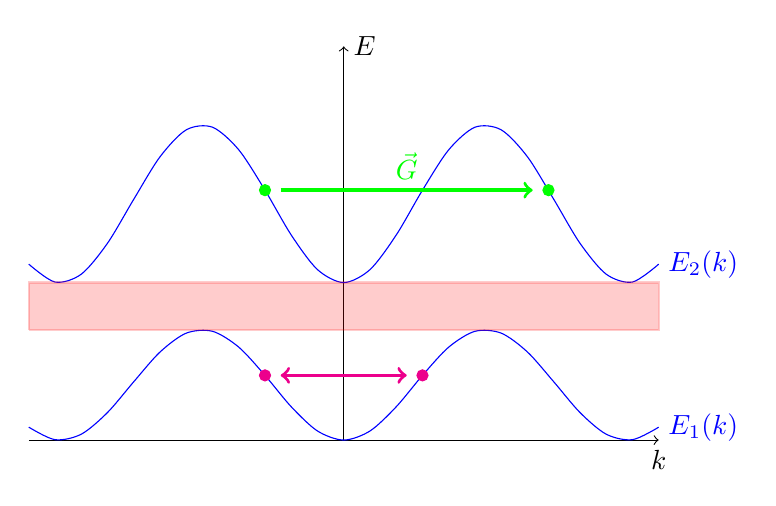
\begin{tikzpicture}
        \draw[->, black] (0, 0) to (0, 5) node[right]{$E$};
        \draw[->, black] (-4, 0) to (4, 0) node[below]{$k$};

        \draw[domain=-4:4, smooth, variable=\x, blue] plot ({\x}, {-0.7*cos(\x*100)+0.7}) node[right]{$E_1(k)$};
        \draw[domain=-4:4, smooth, variable=\x, blue] plot ({\x}, {-cos(\x*100)+3}) node[right]{$E_2(k)$};

        \filldraw[-, draw=red, fill=red, opacity=0.2, thick] (-4, 1.4) to (-4, 2) to (4, 2) to (4, 1.4) to (-4, 1.4);

        \filldraw[green]	(-1, {-cos(-100)+3}) circle (2pt)
							(2.6, {-cos(-100)+3}) circle (2pt);
		\draw[->, green, very thick]	(-0.8, {-cos(-100)+3}) to node[above]{$\vec{G}$} (2.4, {-cos(-100)+3});

		\filldraw[magenta]	(-1, {-0.7*cos(-100)+0.7}) circle (2pt)
							(1, {-0.7*cos(-100)+0.7}) circle (2pt);
		\draw[<->, magenta, very thick]	(-0.8, {-0.7*cos(-100)+0.7}) to (0.8, {-0.7*cos(-100)+0.7});
    \end{tikzpicture}
    \caption{Energy band diagram}
    \label{fig:energybandiagram}
\end{figure}
The wave functions are also periodic in k-space. Thus if we take the green point and translate that on the wave, that point has the same wave, this is translational symmetry (section \ref{sec:property1}). We also notice inversion symmetry, depicted in magenta (section \ref{sec:property2}).
